\normalfont\normalsize
\chapter{Software Implementation}

Our solution is divided into different modules that run independently but communicate with each other to achieve the main goal. The separation of software modules allows future features to be added easily.

There are multiple applications, running on the SparrowDongle and SparrowV3.2, running on the Parrot AR.Drone and a modified instance of the FreeFlight 2.0 application running an Android phone. The connection between them is presented in figure~\ref{fig:arhitecture}.

The SparrowDongle gateway is always in a listen-for-data state and dumps any data it receives on the virtual serial port emulated over USB. When it receives a data packet, it sends back an ACK message to let the SparrowV3.2 nodes know that they can begin sending the entire stored data to the it.

The SparrowV3.2 node is periodically sending a small data packet to check if a gateway is available. It stores the data accumulated during the period when no reply is received. When it receives the ACK message from a mobile gateway it starts sending the previously stored data to the gateway. The data can vary, from sensor readings to debugging information used to check the state of the Wireless Sensor Network.

The data gathered by the gateway is saved into different files in the Parrot AR.Drone's internal memory. The files also contain information such as the node identification tag and time of the transfer. The data can be accessed at any time by any device that connects to the drone's wireless network on port 4242 via FTP.

The drone also processes some of the collected data to provide real time HUD information, such as signal strength, last connection time and number of discovered nodes. This information is sent to the controlling device through a socket connection. The controlling device, PC or Android, gathers that information and displays it to the user. 

\clearpage

\begin{figure}[ht]
\begin{center}
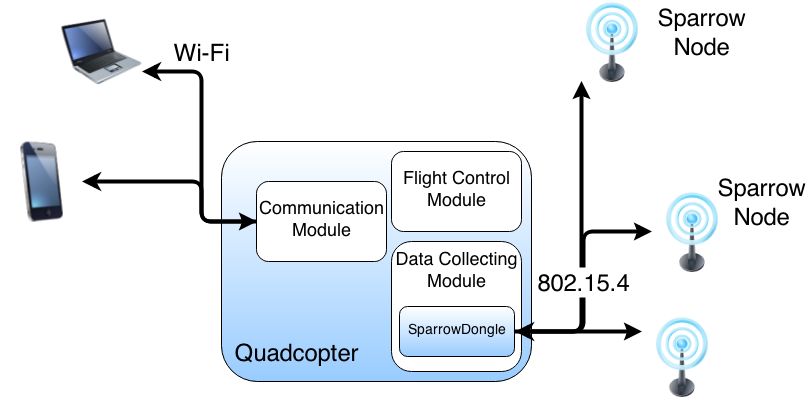
\includegraphics[width=0.9\textwidth]{img/organigrama.png}
\end{center}
\caption{\small \itshape{Modules running on the drone and their connections}}
  \label{fig:arhitecture}
\end{figure}

%change title for drone modules
\section{Drone modules}

\subsection{The USB Module}

The default software with which the drone is delivered does not implicitly recognize the dongle. This behavior was expected because the drone runs a stripped down version of Linux. In order for the drone to recognize the dongle, a module had to be compiled for the specific CPU architecture and operating system that were installed on the drone.

The required module is called cdc\_acm\cite{cdcacm}. This module is responsible for emulating serial ports over USB. The module creates a file, named /dev/ttyACM0, linked with the dongle, which can be read just like any other file.

\subsection{The Debug Module}
 
When performing modification to the existing code, debugging support can greatly speed up the development process. This module allows for displaying control message to the user console even when the process is running in the background. If the messages are always activated, they can slow down the execution speed of the entire application.

In order to see debugging messages, the debug option must be activated and the simple command from listing~\ref{lst:cmd} must be run.

%adauga referinta la listing in text
\lstset{ literate={\$}{{\$}}1, numbers=none,  nolol=false,caption=Simple display message command,label=lst:cmd}
\begin{lstlisting}
p=$(pidof read) && strace -p $p
\end{lstlisting}

Enabling the debug option is just a matter of setting the $DEBUG\_ON$ constant to the value 1, recompiling and uploading the code to the drone. The constants needed for debugging are shown in listing~\ref{lst:debug}.

%adauga referinta la listing in text
\lstset{numbers=none, mathescape=true, nolol=false,caption=Debug and timing defines,label=lst:debug}
\begin{lstlisting}
/* activates/deactivates printf debug information*/
#define DEBUG_ON 0
/* delay time in microseconds*/
#define DELAY_US 100000

/* time in milliseconds since connecting display the node*/
#define TIME_DELTA 45000
#define DEBUG_PRINT(a...) { if(DEBUG_ON) printf(a); }
\end{lstlisting}

In certain parts of the modules a delay is needed in order to wait for an action to be executed. The value $DELAY\_US$ can be changed to any value, but you must be careful in doing so. A small delay sends data more often but it uses a lot of processing power. A big delay could be too slow for the data to be usable. We have chosen a delay of 100 ms, for 10 data updates per second.

Also, the nodes are memorized for the period $TIME\_DELTA$. During this period, the node will be saved and informations about it will be sent to the user. If after $TIME\_DELTA$, no new data has been received from the node, it is deleted from the list.

\subsection{The Data Collecting Module}

The module saves the collected data into the drone's internal memory and pases the data on to the communication module, which displays on the controller interface certain data items like: the number of nodes currently connected to the dongle, the signal strength, dongle connection status etc.

This module contains some extra features that are designed to make the solution more user friendly and easier to extend in the future.

\subsection{Modules intercommunication}

The memory area in which the information sent to the user is saved is shared between this module and the communication module. The interaction method between these two modules resembles the consumer-producer problem, where the Data Collecting Module is represented by the producer and the Communication Module is represented by the consumer.

A important issue with this approach is synchronization and the avoidance of data races. These are prevented with the use of a mutex construct that only allows one thread at a time to access the data. Example is depicted in listing~\ref{lst:mutex}.

\lstset{numbers=none, mathescape=true, nolol=false,caption=Data Collection use of mutex,label=lst:mutex}
\begin{lstlisting}
pthread_mutex_lock(&data_lock);
add_node_data(get_current_timestamp(),read_data + 7);
pthread_mutex_unlock(&data_lock);
\end{lstlisting}

Similarly, the mutex is used in the Communication Module when it consumes data.


\subsection{Fault tolerance}

Because the Dongle is connected to an USB port on a machine that has a lot of vibrations, it might disconnect / reconnect for a very short period of time. This module has been designed to cope with multiple USB disconnects and reconnects without the need to reset the drone. This information is vital, because you can check if the dongle is still connected to the drone without the need to inspect it visually or to connect to a debug terminal.

Besides the possible USB dongle disconnects, an out of range signal may be experienced. If this happens, the drone will hover until the connection is reestablished.

\subsection{The Communication Module}

All of the information gathered by the Data Collecting Module would be useless if it cannot be accessed easily.

This module, as the name suggests, handles the communication of this crucial information back to the user.

Being a different module, with different attributions than the Data Collecting Module, it has an entire Linux process dedicated to it for 3 important reasons:
\begin{enumerate}

\item The approach of having a process per module allows the modules to run independently of each other.
\item The Data Collecting Module can collect the data from the Dongle as soon as this is available.
\item If the Communication Module stops working, the Data Collecting Module can keep collecting data, so complete failure of the system is avoided.
\item System processes can be restarted in case of failure.

\end{enumerate}

\subsection{Socket with connection reset}

The communication is done through socket connections listening on port 8888. The server running on the drone accepts only one connection at a time.

If a connected client decides to disconnect before or while a write operation is in progress, a $SIGPIPE$ error signal will be thrown, stopping all the modules. This is prevented by ignoring the signal, forcing the write action to return a $EPIPE$, and exiting gracefully.

The main process will use the callback \text{ accept\_socket\_connection} to reestablish a new connection. Once a connection is established, it will send information once every $DELAY\_US$ microseconds. The program was configured and tested with a 100ms wait period that translates to ten updates per second.

This delay is required because if there was no delay the communication would occupy too much processor time both on the drone and on the controlling device.

\subsection{JSON Encoding of Data}

JSON \cite{json} is an open-standard that uses text to encode data. It is an alternative to XML. Derived from the JavaScript scripting language, it is a language-independent data format available in most programing languages.

%poti sa raspunzi daca se leaga de data oriented vs document oriented?
JSON is best suitable for this application as a data encode format because it is data oriented, unlike XML which is document oriented. Also, it is very easy to encode because it has a code like structure, the result being smaller than the XML alternative. Another advantage is that all devices can decode it. 

The informations encoded by the drone are:
\begin{itemize}

\item Dongle connection status
\item An array containing node data
\begin{itemize}
‏
	\item Node unique ID
	\item Last connection time of the node to dongle
	\item The power of the received signal

	\end{itemize}
\end{itemize}
 

\section{SparrowV3.2 module}

Due to the communication protocol implemented, the SparrowV3.2 node uses very little power when not connected to
the drone. The solution is similar to the one described by Cardei et al\cite{cardei2005improving}. The Sparrow node sends a small packet at a fixed interval.If the packet is received by the dongle, it will send back a specific ACK just to the node that sent the packet. When the node receives the ACK, it will try to send all the stored data to the drone, starting from the oldest entry to the newest one. The data is stored in a circular linked list of a fixed size. If the list is full, the oldest entity is always replaced by new data.

The drone saves the received data, locally in files that have the name comprised of the timestamp of the current session and the unique id of the node.

\section{Android application modules}
 
\begin{figure}[ht]
\begin{center}
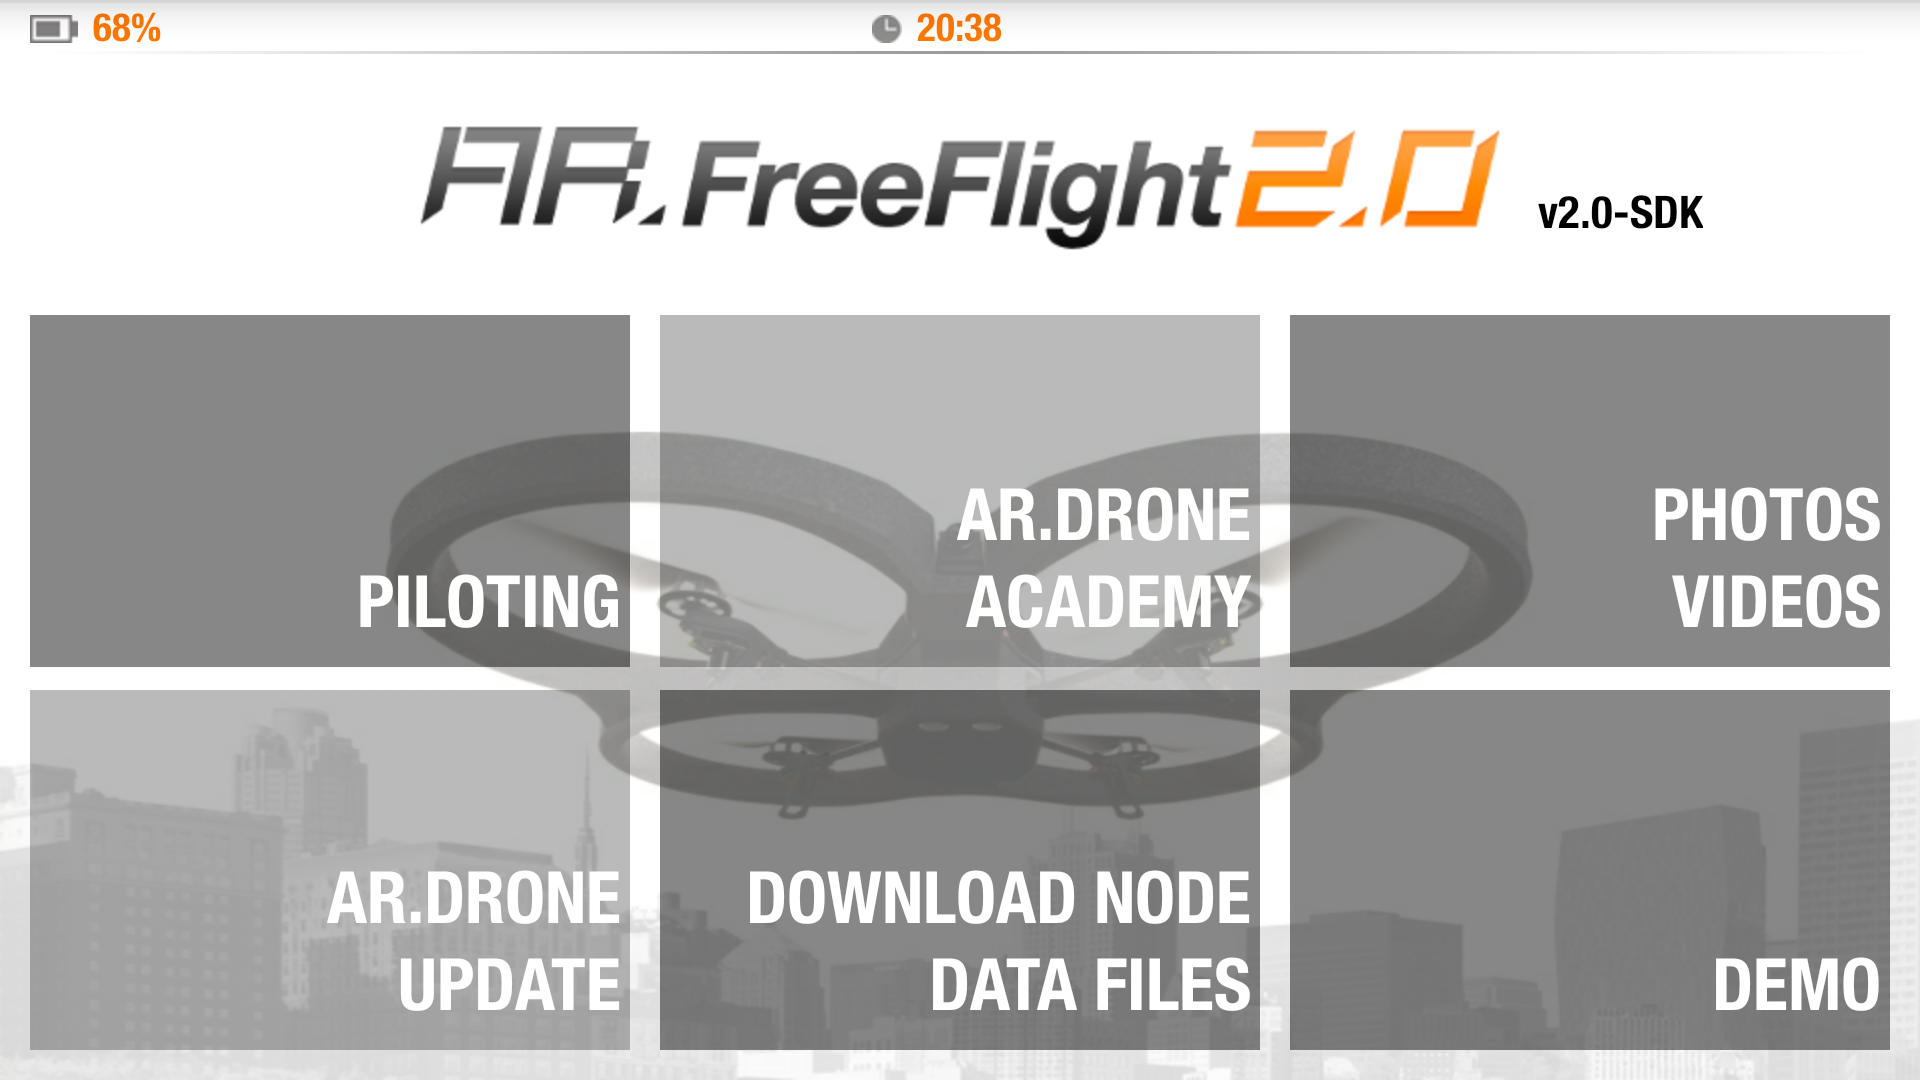
\includegraphics[width=0.9\textwidth]{img/android_app.png}
\end{center}
\caption{\small \itshape{AR Freeflight modified application}}
  \label{fig:moded_app}
\end{figure}

Being an open-source platform we modified the AR Freeflight 2.0 Android application to communicate with the new modules installed on the drone and added a new feature on the main screen, seen in figure~\ref{fig:moded_app}.

Android imposes the use of the background process class AsyncTask when using communication protocols such as http, ftp or sockets. This prevents the UI process from remaining stuck in communication and not responding to user actions.

The class offers 5 very important methods that can be overwritten, 4 running on the main UI process, that prepare data before and after execution, publish progress or simply cancel at any step, and 1 running on the background process.

\subsection{Display information module}
 
\begin{figure}[ht]
\begin{center}
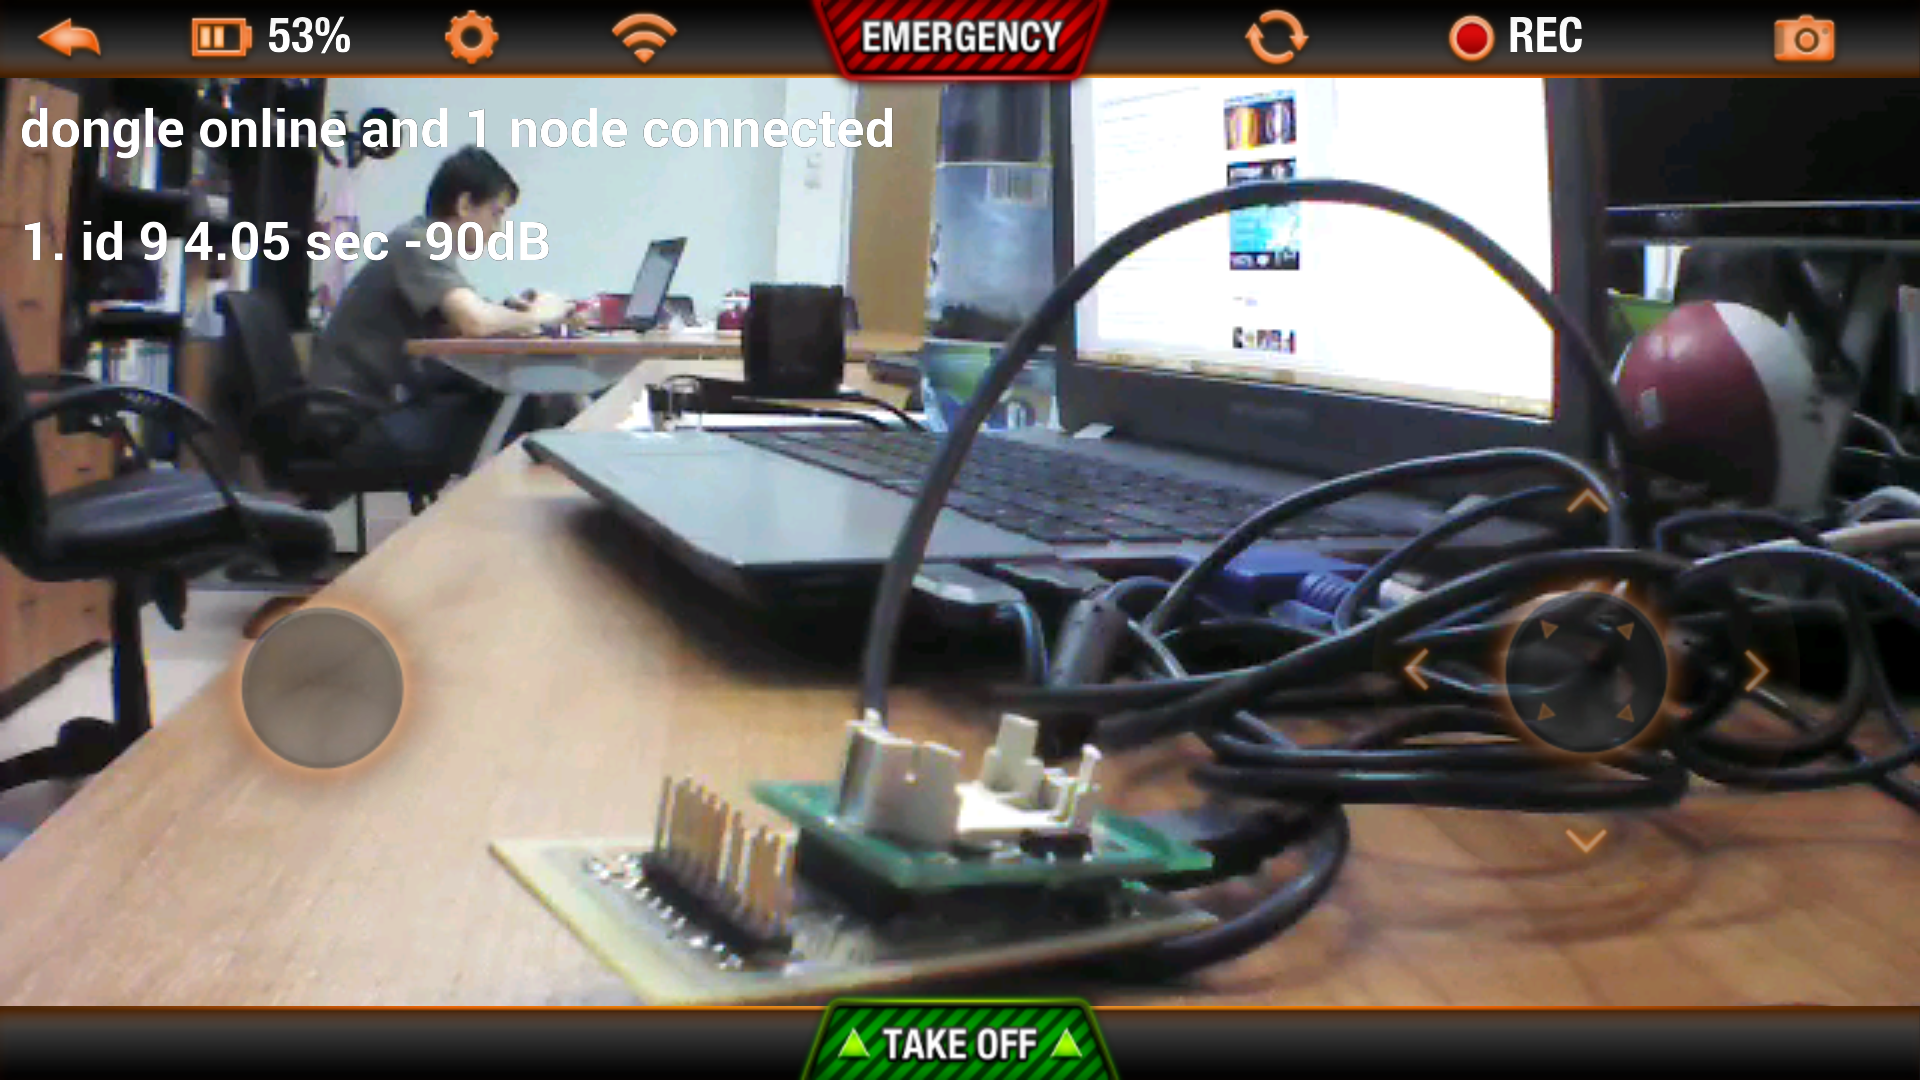
\includegraphics[width=0.9\textwidth]{img/android_info.png}
\end{center}
\caption{\small \itshape{AR Freeflight modified Piloting Screen}}
  \label{fig:pilot}
\end{figure}

The Piloting screen of the application has been modified to display the received data from the drone.

The information displayed is comprised of the state of the dongle, the number of connected nodes and for each node the unique id, last connection time and the signal strength. Up to 9 nodes sorted in descending order after their signal strength are displayed. Figure~\ref{fig:pilot} is an example of how the informations are displayed.

\subsection{FTP communication module}

\begin{figure}[ht]
\begin{center}
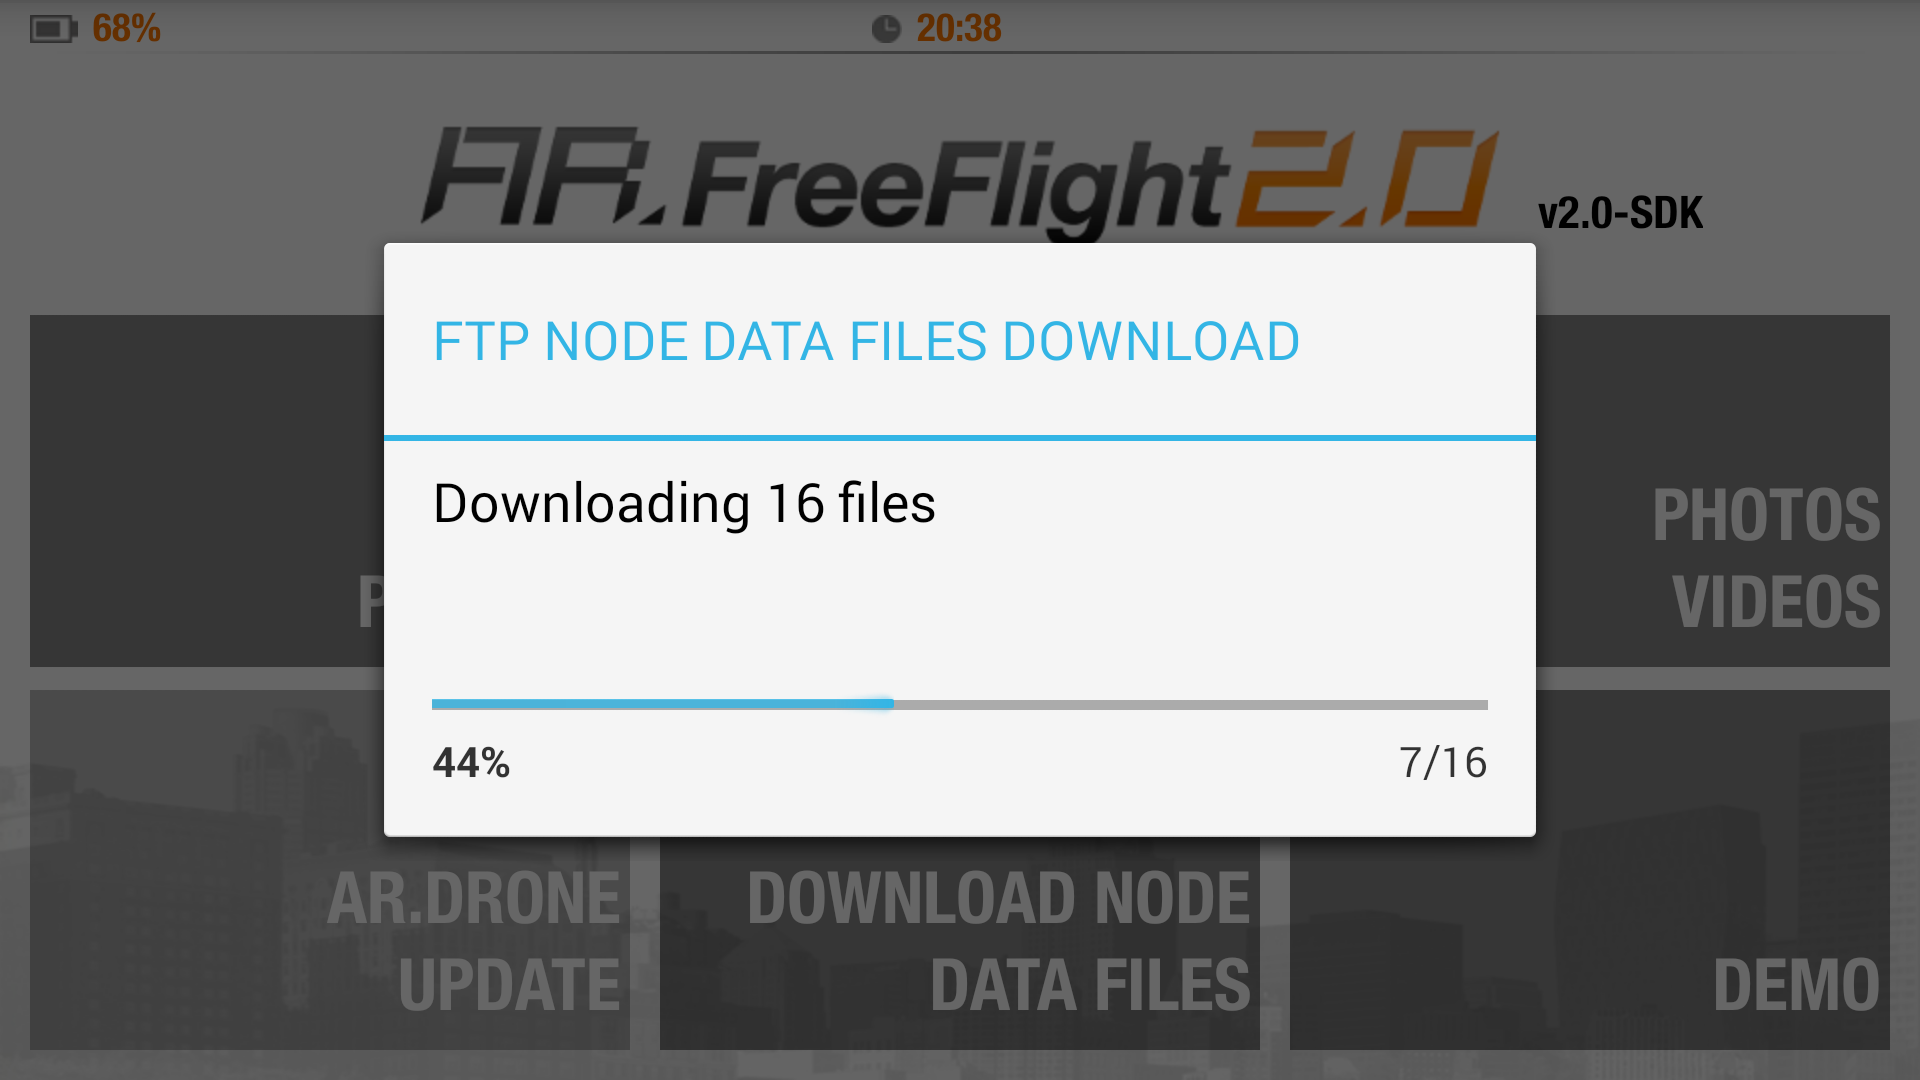
\includegraphics[width=0.9\textwidth]{img/android_ftp.png}
\end{center}
\caption{\small \itshape{AR Freeflight FTP downloading files}}
  \label{fig:ftp}
\end{figure}

The drone has a built-in FTP server that can be configured to allow access to any folders/files on the drone. We have configured the drone so that the folder in which the data is saved can be accessed at any time using port 4242 by any device that has FTP client capabilities. 

This feature was added to the Android application as well, to have a better out of the box experience.

The application will download all the files from the drone to the local storage of the user's Android device and display the progress as in figure~\ref{fig:ftp}.

